\section{Week 2}
\subsection{Objective}
For week 2, we are going to regard the \textit{Bayesian Optimal Design} problem for linear regression, and use this to implement a reference implementation, to be used later.
We can then also explore the effect of different data sizes, different priors and the difference between estimating an objective function through sampling versus calculating it analytically.
\subsection{Theory}
\subsubsection{Bayesian Optimal Design}
Often in scientific contexts as well as other cases, one might have a model that one wishes to strengthen in one way or another using experimental data.
Performing the experiments needed to strengthen one's model can be expensive however, so having an efficient strategy to do such can save important resources.
This is where \textit{Bayesian Optimal Design} comes in.

The Bayesian Optimal Design problem is about finding a design $\B{d}$ from a design space $\B{D}$, that optimizes some kind of utility function.\cite{ryan15} 
For this project, we wish to maximize the expected information gain from the prior to the posterior.
% For this project, that utility function is the mutual information gained from an experiment by measuring at "location" $\B{d}$.\\
To find the optimal design, we want to find a maximizer $\B{d}^*$ defined as such:
\begin{equation}\label{eq:bayesian-optimal}\B{d}^* = \arg \max_{\B{d}\in \B{D}} I(\B{d})\end{equation}
Where $I(\B{d})$ is the \textit{Mutual Information} between the prior and posterior when adjusted for data observed at $\B{d}$.\\
\subsubsection{The Nature of the Mutual Information Metric}
The amount of information of an experiment is often defined as the negative differential entropy defined as such\cite{lindley56}:
\begin{equation}H_x = \int_{X}p(x)\log p(x)dx\end{equation}
Thus, the information known before $\B{y}$ is observed from $\B{d}$ is
\begin{equation}\label{eq:entropy-prior}H_\theta = \int_{\Theta}p(\theta)\log p(\theta)d\theta\end{equation}
and after is
\begin{equation}\label{eq:entropy-posterior}H_{\theta | \B{y}, \B{d}} = \int_{\Theta}p(\theta| \B{y}, \B{d})\log p(\theta| \B{y}, \B{d})d\theta\end{equation}
The gain of information must thus be
\begin{equation}H_\textrm{gain} = H_{\theta | \B{y}, \B{d}} - H_\theta\end{equation}
If we instead regard \eqref{eq:entropy-prior} and \eqref{eq:entropy-posterior} as expectations we get
\begin{equation} = \mathbb{E}_{\theta | \B{y}, \B{d}}[\log p(\theta | \B{y}, \B{d})] - \mathbb{E}_\theta [\log p(\theta )]\end{equation}
Before we perform the experiment, we do not know what the outcome will be. Instead, we'll just regard the expected outcome by taking the expectation over the observed evidence $\B{y} | \B{d}$:
\begin{equation} \label{eq:mi-bad}\mathbb{E}_{\B{y} | \B{d}}[H_\textrm{gain}]  = \mathbb{E}_{\B{y} | \B{d}}[\mathbb{E}_{\theta | \B{y}, \B{d}} [\log(p(\theta | \B{y}, \B{d}))] - \mathbb{E}_{\theta}[\log(p(\theta))]]\end{equation}
This expression is called the \textit{Mutual Information} between the prior and posterior, and will be denoted $I(\B{d})$.\\
% It is widely seen in the litterature \cite{lindley56}, \cite{ryan15} that the two inner expectation is put under one, namely $\mathbb{E}_{\theta}$, giving a slightly different definition which is closer tied to the KL-divergence\footnote{This new definition is not entirely equivalent to the one purely based on information. I have included both definitions to show how Mutual Information is related to information theory, as shown in \citet{lindley56}}.
We can also rewrite the expectations as such using Bayes' rule and that $\B{\theta}$ is independent from $\B{y}|\B{d}$:
\begin{equation}\label{eq:mi}I(\B{d})  = \mathbb{E}_{\B{y}|\B{d}}[\mathbb{E}_{\theta| \B{y}, \B{d}} [\log(p(\theta | \B{y}, \B{d}))]] - \mathbb{E}_{\theta}[\log(p(\theta))]\end{equation}
\begin{equation}= \mathbb{E}_\B{\theta}[\mathbb{E}_{\B{y}| \theta, \B{d}} [\log(p(\theta | \B{y}, \B{d}))]] - \mathbb{E}_{\theta}[\log(p(\theta))]\end{equation}
\begin{equation}= \mathbb{E}_\B{\theta}[\mathbb{E}_{\B{y}| \theta, \B{d}} [\log(p(\theta | \B{y}, \B{d}))] - \log(p(\theta))]\end{equation}
\begin{equation}= \mathbb{E}_\B{\theta}[\mathbb{E}_{\B{y}| \theta, \B{d}} [\log(p(\theta | \B{y}, \B{d})) - \log(p(\theta))]]\end{equation}
We can now use Bayes' rule to get

% We can put a new interpretation upon this by expanding equation \ref{eq:mi} using Bayes' rule:
\begin{equation} I(\B{d})  = \mathbb{E}_{\B{\theta}}[\mathbb{E}_{\B{y} | \theta, \B{d}} [\log(p(\B{y} | \B{\theta}, \B{d})) - \log(p(\B{y}|\B{d}))]]\end{equation} 
Then we can use that $\frac{p(\B{y}, \B{\theta}|\B{d})}{p(\theta)}=p(\B{y| \theta, \B{d}})$:
\begin{equation} I(\B{d})  = \mathbb{E}_{\B{\theta}}[\mathbb{E}_{\B{y} | \theta, \B{d}} [\log\left(\frac{p(\B{y}, \B{\theta}|\B{d})}{p(\theta)}\right) - \log(p(\B{y}|\B{d}))]]\end{equation}
\begin{equation}= \mathbb{E}_{\B{\theta}}[\mathbb{E}_{\B{y} | \theta, \B{d}} [\log\left(\frac{p(\B{y}, \B{\theta}|\B{d})}{p(\theta)p(\B{y}|\B{d})}\right)]]\end{equation}
$$ = \textsc{KL}(p(\B{y}, \theta | \B{d})|| p(\theta)p(\B{y}|\B{d}))$$
Two random variables $X$ and $Y$ are said to be \textit{independent} if the product of their distributions is the same as their joint distribution i.e.
\begin{equation}p(X,Y) = p(X)p(Y)\end{equation}
Thus, the Mutual Information metric measures how close the prior and the evidence are to be independent. 
If $\B{d}$ is picked such that the prior has a high probability of being able to predict $\B{y}|\B{d}$, then the mutual information is going to be close to 0. 
If, on the contrary, $\B{d}$ is picked such that the prior has a low probability of being able to predict $\B{y}|\B{d}$, the mutual information is going to be large.
Thus one could expect that an optimizer would prefer to pick a $\B{d}$ within an area where the prior is not very representative of the underlying generating function.
Of course, in an experimental design context we do not have access to this underlying function as we might not be able to simulate experiments accurately. Instead, the expectation expressions in \eqref{eq:mi}
makes it such that we only regard the expected information gain for any given underlying function.
For the rest of this project, we will regard the definition of mutual information as in \eqref{eq:mi}.

\subsubsection{Evaluating the Mutual Information through sampling}
Without using any assumptions about the nature of our model or data, we can utilize Monte Carlo sampling to obtain an accurate estimate on the expectations in \eqref{eq:mi}.
First we'll use that the prior is independent of $\B{y}|\B{d}$ to get
\begin{equation}
  I(\B{d}) = \mathbb{E}_\B{\theta}[\mathbb{E}_{\B{y}| \theta, \B{d}} [\log(p(\theta | \B{y}, \B{d}))]] - \mathbb{E}_{\theta}[\log(p(\theta))]
\end{equation}
\begin{equation}
  = \mathbb{E}_\B{\theta}[\mathbb{E}_{\B{y}| \theta, \B{d}} [\log(p(\theta | \B{y}, \B{d}))]] - H_\theta
\end{equation}
Then we can use that entropy of multivariate Gaussian distributions has a closed form solution:
\begin{equation}
  = \mathbb{E}_\B{\theta}[\mathbb{E}_{\B{y}| \theta, \B{d}} [\log(p(\theta | \B{y}, \B{d}))]] - \frac{1}{2}\ln \det (2\pi e\Sigma_\theta)
\end{equation}
Then we can sample the nested expectations. For $N$ samples of $\theta \sim p(\theta)$ and $M$ samples of $\B{y}_i \sim p(\B{y}_i | \theta_i, \B{d})$ this looks like
\begin{equation}
  \label{eq:mi-sampled}I(\B{d}) \approx \frac{1}{NM}\sum_{i=0}^N\sum_{j=0}^M(\log (p(\theta_i | \B{y}_{ij}, \B{d}))) - \frac{1}{2}\ln \det (2\pi e\Sigma_\theta)
\end{equation}

\subsubsection{Stochastic Optimization}
For the sampling approach here, and in the rest of the project, we will use a stochastic gradient descent algorithm to perform the optimization necessary to solve \eqref{eq:bayesian-optimal}.
From some starting point $\B{d}_0$, iteratively update $\B{d}_i$ by
\begin{equation}
  \B{d}_i = \B{d}_{i-1} + \alpha \frac{1}{10^c + i \times 10^{-\beta}} \nabla_{\B{d}} I(\B{d}_{i-1})
\end{equation}
where $\alpha, \beta, c \in \mathbb{R}$ are hyper-parameters that ensures a slow convergence to tailor the variance that occurs when using Monte Carlo methods.

\subsection{Implementation}
The mutual information metric can be implemented using the sampling method like so:
\begin{minted}{python}
def mutual_information(d):
    l = len(d)
    M = 2
    N = 5
    samples = []
    thetas = np.random.multivariate_normal(mu_prior, cov_prior, size=N)
    for theta in thetas:
        ys = ((np.tile(augment_d(d), (M, 1, 1)) @ theta).T + (noise * np.eye(len(d))) @ np.random.randn(len(d), M)).T
        for y in ys:
            mu_post, cov_post = analytical_posterior_params(augment_d(d), y)
            val = stable_multivariate_gaussian_logpdf(theta, mu_post, cov_post) - 0.5 * np.log(np.linalg.det(2*np.pi*np.e*cov_prior))
            samples.append(val)
    return 1/(N * M) * np.sum(samples)
\end{minted}

Finding the gradient can be done using \texttt{autograd.grad}. 
An example of this can be seen in this implementation of the gradient descent algorithm:
\begin{minted}{python}
def optimize(f, d0, alpha, beta, c, iterations):
  d = d0
  g = grad(f)
  for i in range(iterations):
    d = d + alpha / (10**c + i * 10**(-beta)) * g(d)
  return d
\end{minted}

\subsubsection{Optimizing over 2-d Matrices}
A small, but important note in these implementations is that $\B{d}$ is two-dimensional.
To make computation of gradients and optimization much easier, whenever we are in the context of the optimization algorithm, we will regard $\B{d}$ and the gradient as vectors of the shape
$$\B{d}_v = \begin{bmatrix}\B{d}_{1,1} \\ \vdots  \\ \B{d}_{1,d} \\ \B{d}_{2,1} \\ \vdots \\ \B{d}_{\ell, d} \end{bmatrix}$$
Whenever we are in the context of Mutual information, we will regard $\B{d}$ as a matrix. The following helper functions can thus be used to flatten and reconstruct the matrices as needed:
\begin{minted}{python}
def encode_d(d): # matrix to vector
    return d.flatten()
def decode_d(encoded_d, dim=2): # vector to matrix
    return encoded_d.reshape(int(len(encoded_d)/dim), dim)
\end{minted}

\subsubsection{Implementing the log-PDF of Multivariate Normal Distribution}
Optimizing over this Mutual Information objective function means calculating the gradient of it. 
We will use \texttt{autograd.grad} to do this, which necessitates implementing the log-PDF of the multivariate normal distribution by hand, 
since the one supplied by \texttt{autograd.scipy.stats} does not handle the case where the mean and covariance carries information about the computation graph, which also will be necessary later.\\
The log-PDF of the multivariate normal distribution is given by:
\begin{equation}
  \log \mathcal{N}(x; \mu, \Sigma) = -\frac{1}{2}(n\log(2\pi) + \log(\det(\Sigma)) + (x - \mu)^T\Sigma^{-1}(x - \mu))
\end{equation}
It is important that this implementation is numerically stable and efficient, since it will be used a lot.
The following implementation is used:
\begin{minted}{python}
def stable_multivariate_gaussian_logpdf(x, mu, cov):
    n = cov.shape[-1]
    x_mu = x - mu
    _, log_det = np.linalg.slogdet(cov)
    cov_inv = np.linalg.inv(cov)
    prod = x_mu.T @ cov_inv @ x_mu
    log_prob = -0.5 * (n * np.log(2 * np.pi) + log_det + prod)
    return log_prob
\end{minted}
\subsection{Results}
If we regard the problem with $\ell = 10$ data points and $d=2$ dimensions with a zero-mean prior with identity prior covariance, 
we will see data closer to the optimum be spread out wider and more evenly in the parameter space.
This can be seen if one regards \eqref{eq:mi-sampled}:
If $\B{d}$ is picked such that $\B{d}\theta_i$ has a high probability of being a small number, then
$\B{d}\theta_i + \sigma^2_\B{y}\B{z}_j$ is going to get dominated by the noise term $\sigma^2_\B{y}\B{z}_j$.
Thus, the log-posterior $\log p(\theta_i | \B{d}\theta_i + \sigma^2_\B{y}\B{z}_j, \B{d})$ will be smaller.
If on the other hand, $\B{d}$ is picked such that $\B{d}\theta_i$ has a high probability of being a large number, then $\B{d}\theta_i$ is going to dominate the noise term
and the posterior has a higher probability of being a large number.\\
In Figure \ref{fig:mi-2d}, we can see if the start position consists of 10 data points on top of each other at $(0,0)$, they will swiftly move to a more spread out formation.\\
If we choose a zero-mean prior with an identity covariance, the points will spread out instantly from the center. If we choose a non-zero mean and non-identity covariance, 
the gradient seems to become more steep such that some of the points can move away quite fast.
If we insert a regularization factor $\mathcal{L} = 10^{-2}\times |\B{d}|^2$, the points will diverge confidently from the start position until some point, where they will start to stutter and not move much more.

\begin{figure}
  \centering
  \begin{subfigure}{.5\textwidth}
    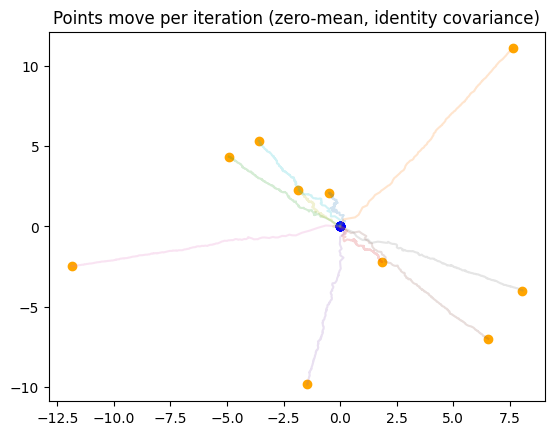
\includegraphics[width=0.8\textwidth]{week2/mi-2d-unit.png}
  \end{subfigure}%
  \begin{subfigure}{.5\textwidth}
    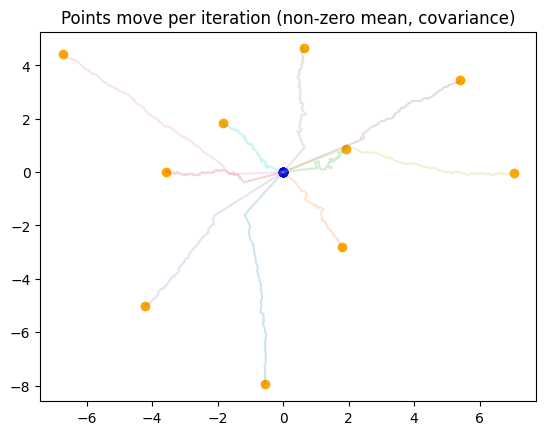
\includegraphics[width=0.8\textwidth]{week2/mi-2d-non-unit.png}
  \end{subfigure}
  \begin{subfigure}{.5\textwidth}
    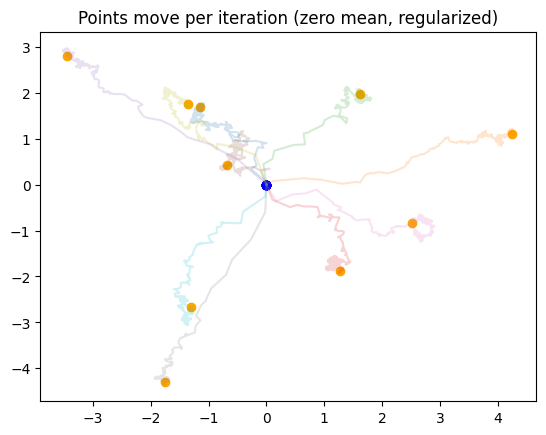
\includegraphics[width=0.8\textwidth]{week2/mi-2d-reg.png}
  \end{subfigure}
  \centering
  \caption{Points in $\B{d}$-space moving from their start position (blue) and increasingly away from it.}
  \label{fig:mi-2d}
\end{figure}
\begin{figure}
  \centering
  \begin{subfigure}{.5\textwidth}
    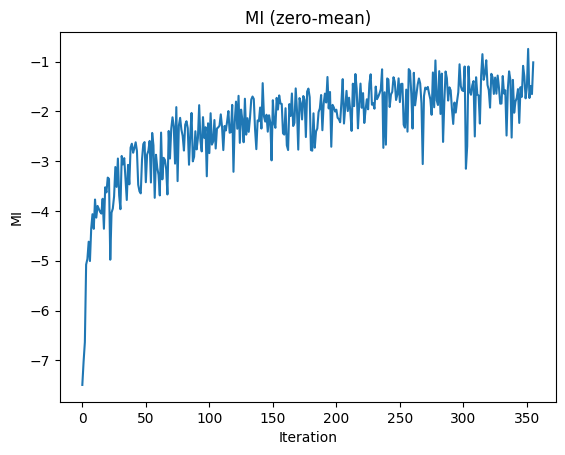
\includegraphics[width=0.8\textwidth]{week2/mi-over-time-zero.png}
  \end{subfigure}%
  \begin{subfigure}{.5\textwidth}
    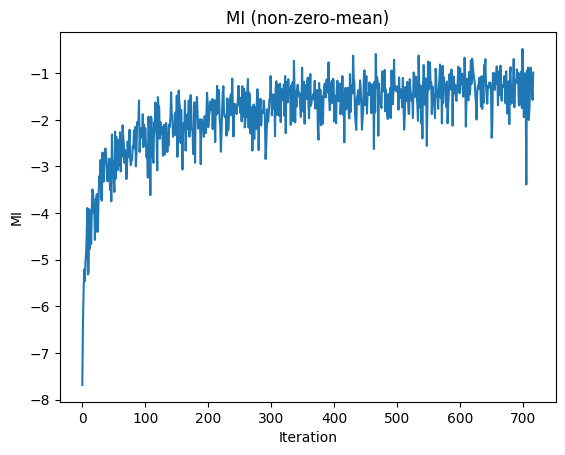
\includegraphics[width=0.8\textwidth]{week2/mi-over-time-non-zero.png}
  \end{subfigure}
  \begin{subfigure}{.5\textwidth}
    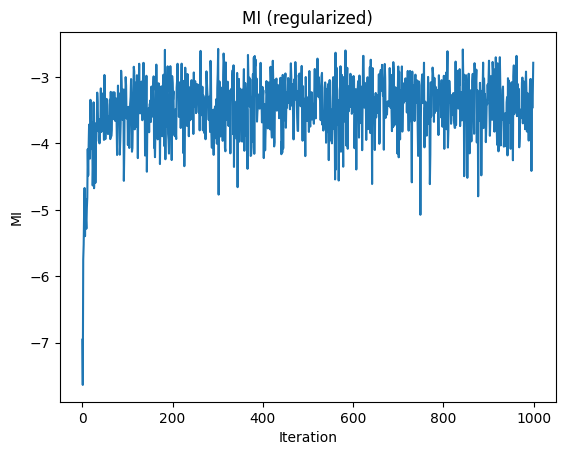
\includegraphics[width=0.8\textwidth]{week2/mi-over-time-reg.png}
  \end{subfigure}
  \centering
  \caption{Convergence of each of the plots from Figure \ref{fig:mi-2d}}
  \label{fig:mi-over-time}
\end{figure}
Thus we've seen how optimizing over the Mutual Information metric can help find solutions to the Bayesian Optimal Design problem.
Now we will move on to exploring how to solve regression problems, even when analytical solutions are not available with the hopes of opening up our Mutual Information optimizer to all kinds of models.
